% !TeX root = main.tex

\hypertarget{maxima-and-minima}{%
\section{Maxima and Minima}\label{maxima-and-minima}}

\begin{definition}

Let \(f\) be a function defined over an interval \(I\) and \(c\) a
number in \(I\). We say \(f\) has an \textbf{\emph{absolute maximum}} on
\(I\) at \(c\) if \(f(c)\ge f(x)\) for all \(x\) in \(I\). We say \(f\) has
an \textbf{\emph{absolute minimum}} on \(I\) at \(c\) if \(f(c) \le f(x)\)
for all \(x\) in \(I\). If \(f\) has an absolute maximum on \(I\) at
\(c\) or an absolute minimum on \(I\) at \(c\), we say \(f\) has an
absolute extremum on \(I\) at \(c\).

\begin{fullwidth}
  \centering
  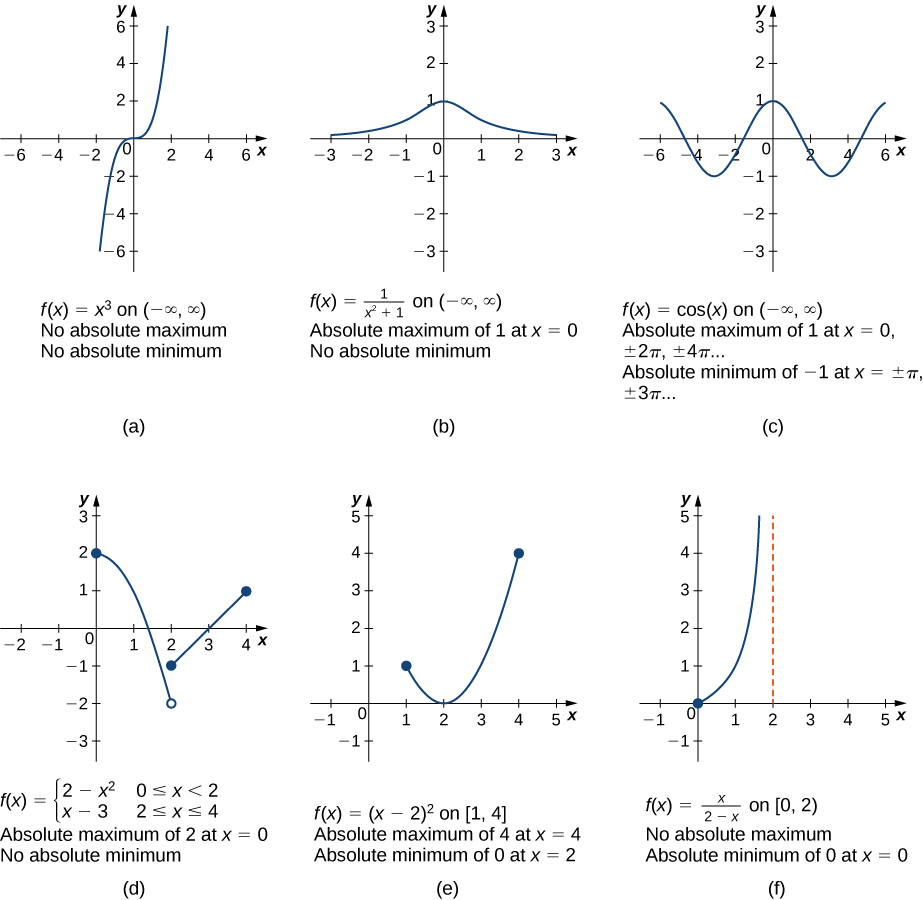
\includegraphics[width=0.8\linewidth]{img/CNX_Calc_Figure_04_03_010.jpeg}
\end{fullwidth}

\end{definition}

\begin{theorem}

\textbf{(Extreme Value Theorem):}

If \(f\) is a continuous function over the closed, bounded interval
\([a,b]\), then there is a point in \([a,b]\) at which \(f\) has an
absolute maximum over \([a,b]\) and there is a point in \([a,b]\) at
which \(f\) has an absolute minimum over \([a,b]\).

\end{theorem}

\begin{definition}

A function \(f\) has a \textbf{local maximum} at \(c\) if there exists
an open interval \(I\) containing \(c\) such that \(I\) is contained in
the domain of \(f\) and \(f(c)\ge f(x)\) for all \(x\) in \(I\). A function
\(f\) has a \textbf{local minimum} at \(c\) if there exists an open
interval \(I\) containing \(c\) such that \(I\) is contained in the
domain of \(f\) and \(f(c) \le f(x)\) for all \(x\) in \(I\). A function
\(f\) has a \textbf{local extremum} at \(c\) if \(f\) has a local
maximum at \(c\) or \(f\) has a local minimum at \(c\).

A local extremum is also known as a relative extremum.

\end{definition}

\begin{theorem}

\textbf{(Fermat's Theorem):} If \(f\) has a local extremum at \(c\) and
\(f\) is differentiable at \(c\), then \(f'(c)=0.\)

\end{theorem}

\begin{definition}

Let \(c\) be an interior point in the domain of \(f\). We say that \(c\)
is a critical point of \(f\) if \(f'(c)=0\) or \(f'(c)\) is undefined.

\begin{fullwidth}
  \centering
  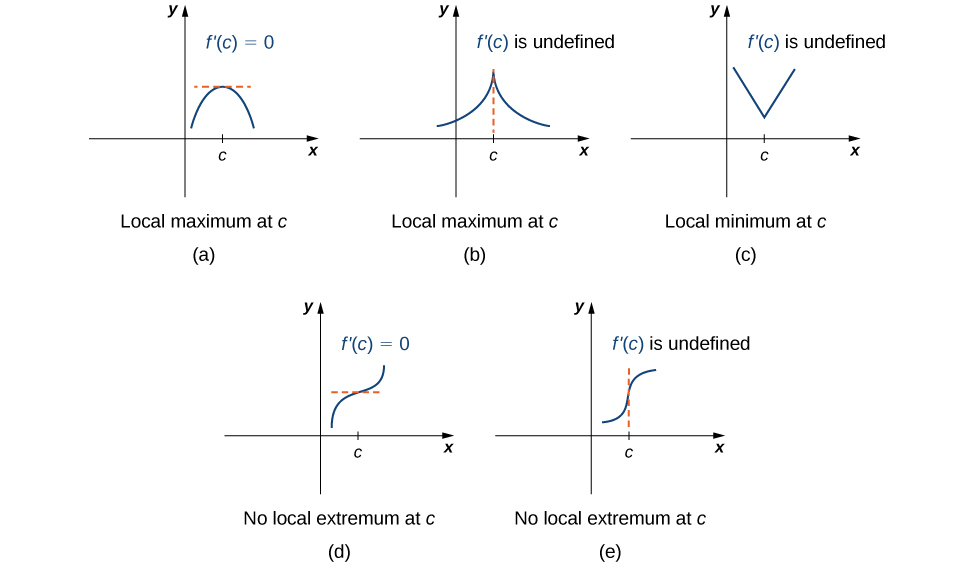
\includegraphics[width=0.8\linewidth]{img/CNX_Calc_Figure_04_03_004.jpeg}
\end{fullwidth}

\end{definition}

\begin{example}

For each of the following functions, find all critical points and
determine whether the function has a local extremum at each of the
critical points.

\begin{enumerate}
\item
  \(f(x)=\frac{1}{3}x^3 - \frac{3}{2}x^2-4x\)
\item
  \(f(x)=\frac{x}{x^2-1}\)
\end{enumerate}

\end{example}

\hypertarget{where-to-locate-absolute-extrema}{%
\subsection{Where to locate absolute
extrema}\label{where-to-locate-absolute-extrema}}

The absolute maximum of a function \(f\) over \(I\) and the absolute
minimum of \(f\) over a closed interval \(I\) must occur at endpoints of
\(I\) or at critical points of \(f\) in \(I\).

\begin{example}

For each of the following functions, find points where the function has
the absolute maximum or absolute minimum over the given interval.

\begin{enumerate}
\item
  \(f(x)= - x^2-2x - 3\) over \([0,4].\)
\item
  \(f(x)=x^2 - 3x^{2/3}\) 2. over \([0,2]\).
\end{enumerate}

\end{example}

\begin{example}

Find the absolute maximum and absolute minimum of the function
\(f(x)=\sin(x)+\cos(x)\).

\end{example}
\vspace*{6\baselineskip}

\begin{example}

Find the absolute maximum and absolute minimum of the function
\[f(x)=|x+1|+|x-1|\quad\text{over}\quad [-3,2].\]

\end{example}
\vspace*{6\baselineskip}

\begin{example}

Find the absolute maximum and absolute minimum of the function
\[f(x)=x\sqrt{4-x^2}.\]

\end{example}
\vspace*{6\baselineskip}

\subsection{Practice}

\begin{exercise}

Find the critical values of the function \[f(x)=3\sqrt{x}+x^2.\]

\end{exercise}
\vspace*{6\baselineskip}

\begin{exercise}

Find the critical values of the function \[f(x)=|x^2-2x-8|.\]

\end{exercise}
\vspace*{6\baselineskip}

\begin{exercise}

Find the absolute maximum and absolute minimum of the function
\[f(x)=4x-x^2\quad\text{over}\quad [-3,6].\]

\end{exercise}
\vspace*{6\baselineskip}

\begin{exercise}

Find the absolute maximum and absolute minimum of the function
\[g(x)=3x+6\sin x \quad\text{over}\quad [0,\pi].\]

\end{exercise}
\vspace*{6\baselineskip}

\begin{exercise}

Find the absolute maximum and absolute minimum of the function
\[h(x)=x^2\sqrt{9x-x^2}.\]

\end{exercise}

